\highlight{placeholder abstract - only for general idea not to be proofread}
\begin{figure}
    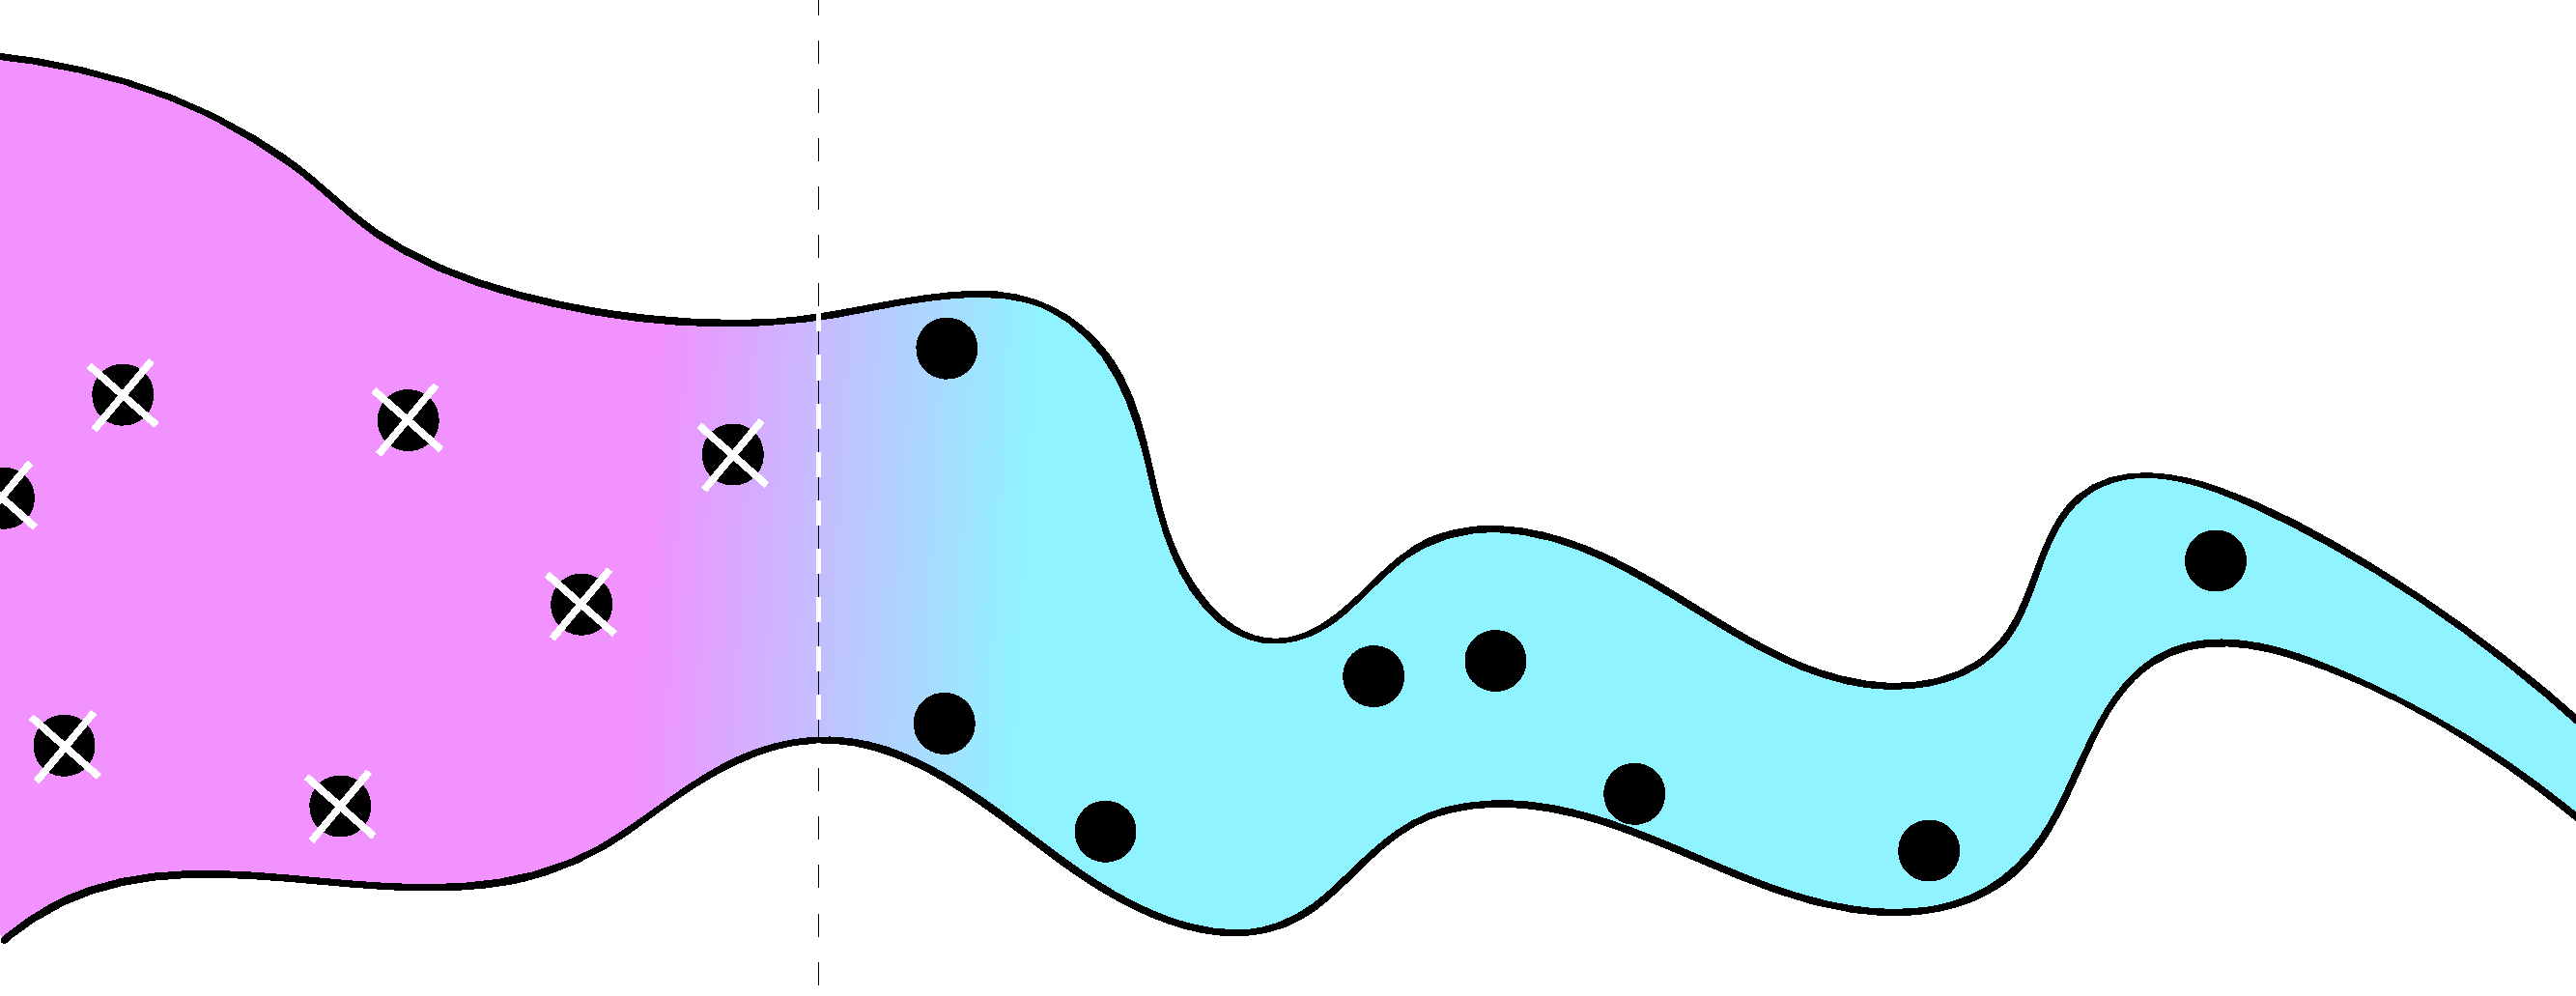
\includegraphics[width=\columnwidth]{picto visual abstract.pdf}
\end{figure}
Estuaries are a challenging for plankton.
Gradients are steep and currents are strong.
Retention mechanisms crucial process for survival.
However, very little experimental and theoretical evidence has been gathered.
We will conduct a model study.
First we will show the importance of retention mechanism for plankton in the Elbe.
Secondly we will study different retention mechanism which are suspected to be applied by organism.
We compare the outcome of the different experiment and judge their effectiveness.

\section*{Introduction}

\subsection*{Why do we care about retention in estuaries?}
\begin{itemize}
    \item Estuaries are important
    \begin{itemize}
        \item high productivity relative to surface area
        \item nutrient source for marine ecosystem
        \item hatching grounds for not only for estuarine but marine species
    \end{itemize}
    %and productive ecosystem - both as fertilizer for marine ecosystems as well as for the global climate system.
    \item Ecosystem strongly "controlled" by primary producer.
    \begin{itemize}
        \item (Do I need to argue/cite something for this?)
    \end{itemize}
    \item Primary producers almost exclusively planktonic. [cite]
          % Suspected reasons: trenching, high velocities on lose soil, high turbidity
    \item strong hydrodynamic currents %and strong chemical gradiants.
    \item "retainment" crucial for survival 
    %for organisms as they would die if washed out to downstream/higher salinity areas.
    \item "swimming" upstream is impossible or too energy expensive for planktonic organisms
    \item However, retainment mechanisms are mostly unknown
    \item Q: How do they survive?
    % as they are hard to study experimentally.
\end{itemize}

\subsection*{Previous studies - aka - what is known}

There are three kind of retention studies: observations, theoretical studies, or modelling studies

\paragraph{observations}
\begin{itemize}
    \item only larger organisms which are not strictly planktonic (fish-larve, mesozooplanktion) [cite]
    \begin{itemize}
        \item found diel migration  [cite]
        \item found tide driven migration
        \item found "sticking" to "ground" [cite]
        \item 
    \end{itemize}
    \item summary: retention indications found for "planktonic" - tho not directly transferable to phytoplankton
\end{itemize}

\paragraph{theoretical}
\begin{itemize}
    \item interesting but study simplistic conditions 
    \item two interesting ones:
    \begin{itemize}
        \item investigation of reproduction threshold under exchange cite
        \item study on "reseeding" due to local upstream currents
    \end{itemize}
    summury: both "outgrowing" and "reseeding" are expected to be possible
\end{itemize}

\paragraph{(particle tracking) models}
\begin{itemize}
    \item only one particle tracking model in estuaries which studies zooplankton
    \item others studies open water or non planktonic organisms i.e. fish
    \item the existing one has mayor drawbacks - e.g. no reproduction
    \item found that sinking and diel migration slows outwashing
    \item non were able to actually study retention in realistic conditions due to technical constraints
\end{itemize}

\paragraph{Summary}
\begin{itemize}
    \item "surrounding" studies have been made
    \item none were able to tackle retention mechanisms themselves
    \item indication for potential mechanisms have been found
    \item we will investigate retention and reseeding mechanism under different plankton migration behavior
\end{itemize}

\section*{Methods}

\subsection*{general model description}
\paragraph{working principle}
\begin{itemize}
    \item particle tracking
    \begin{itemize}
        \item fast
        \item easy to interpret
        \item flexible e.g. allows "individual" processes
        \item realistic representation of motion
    \end{itemize}
\end{itemize}
\begin{figure}
    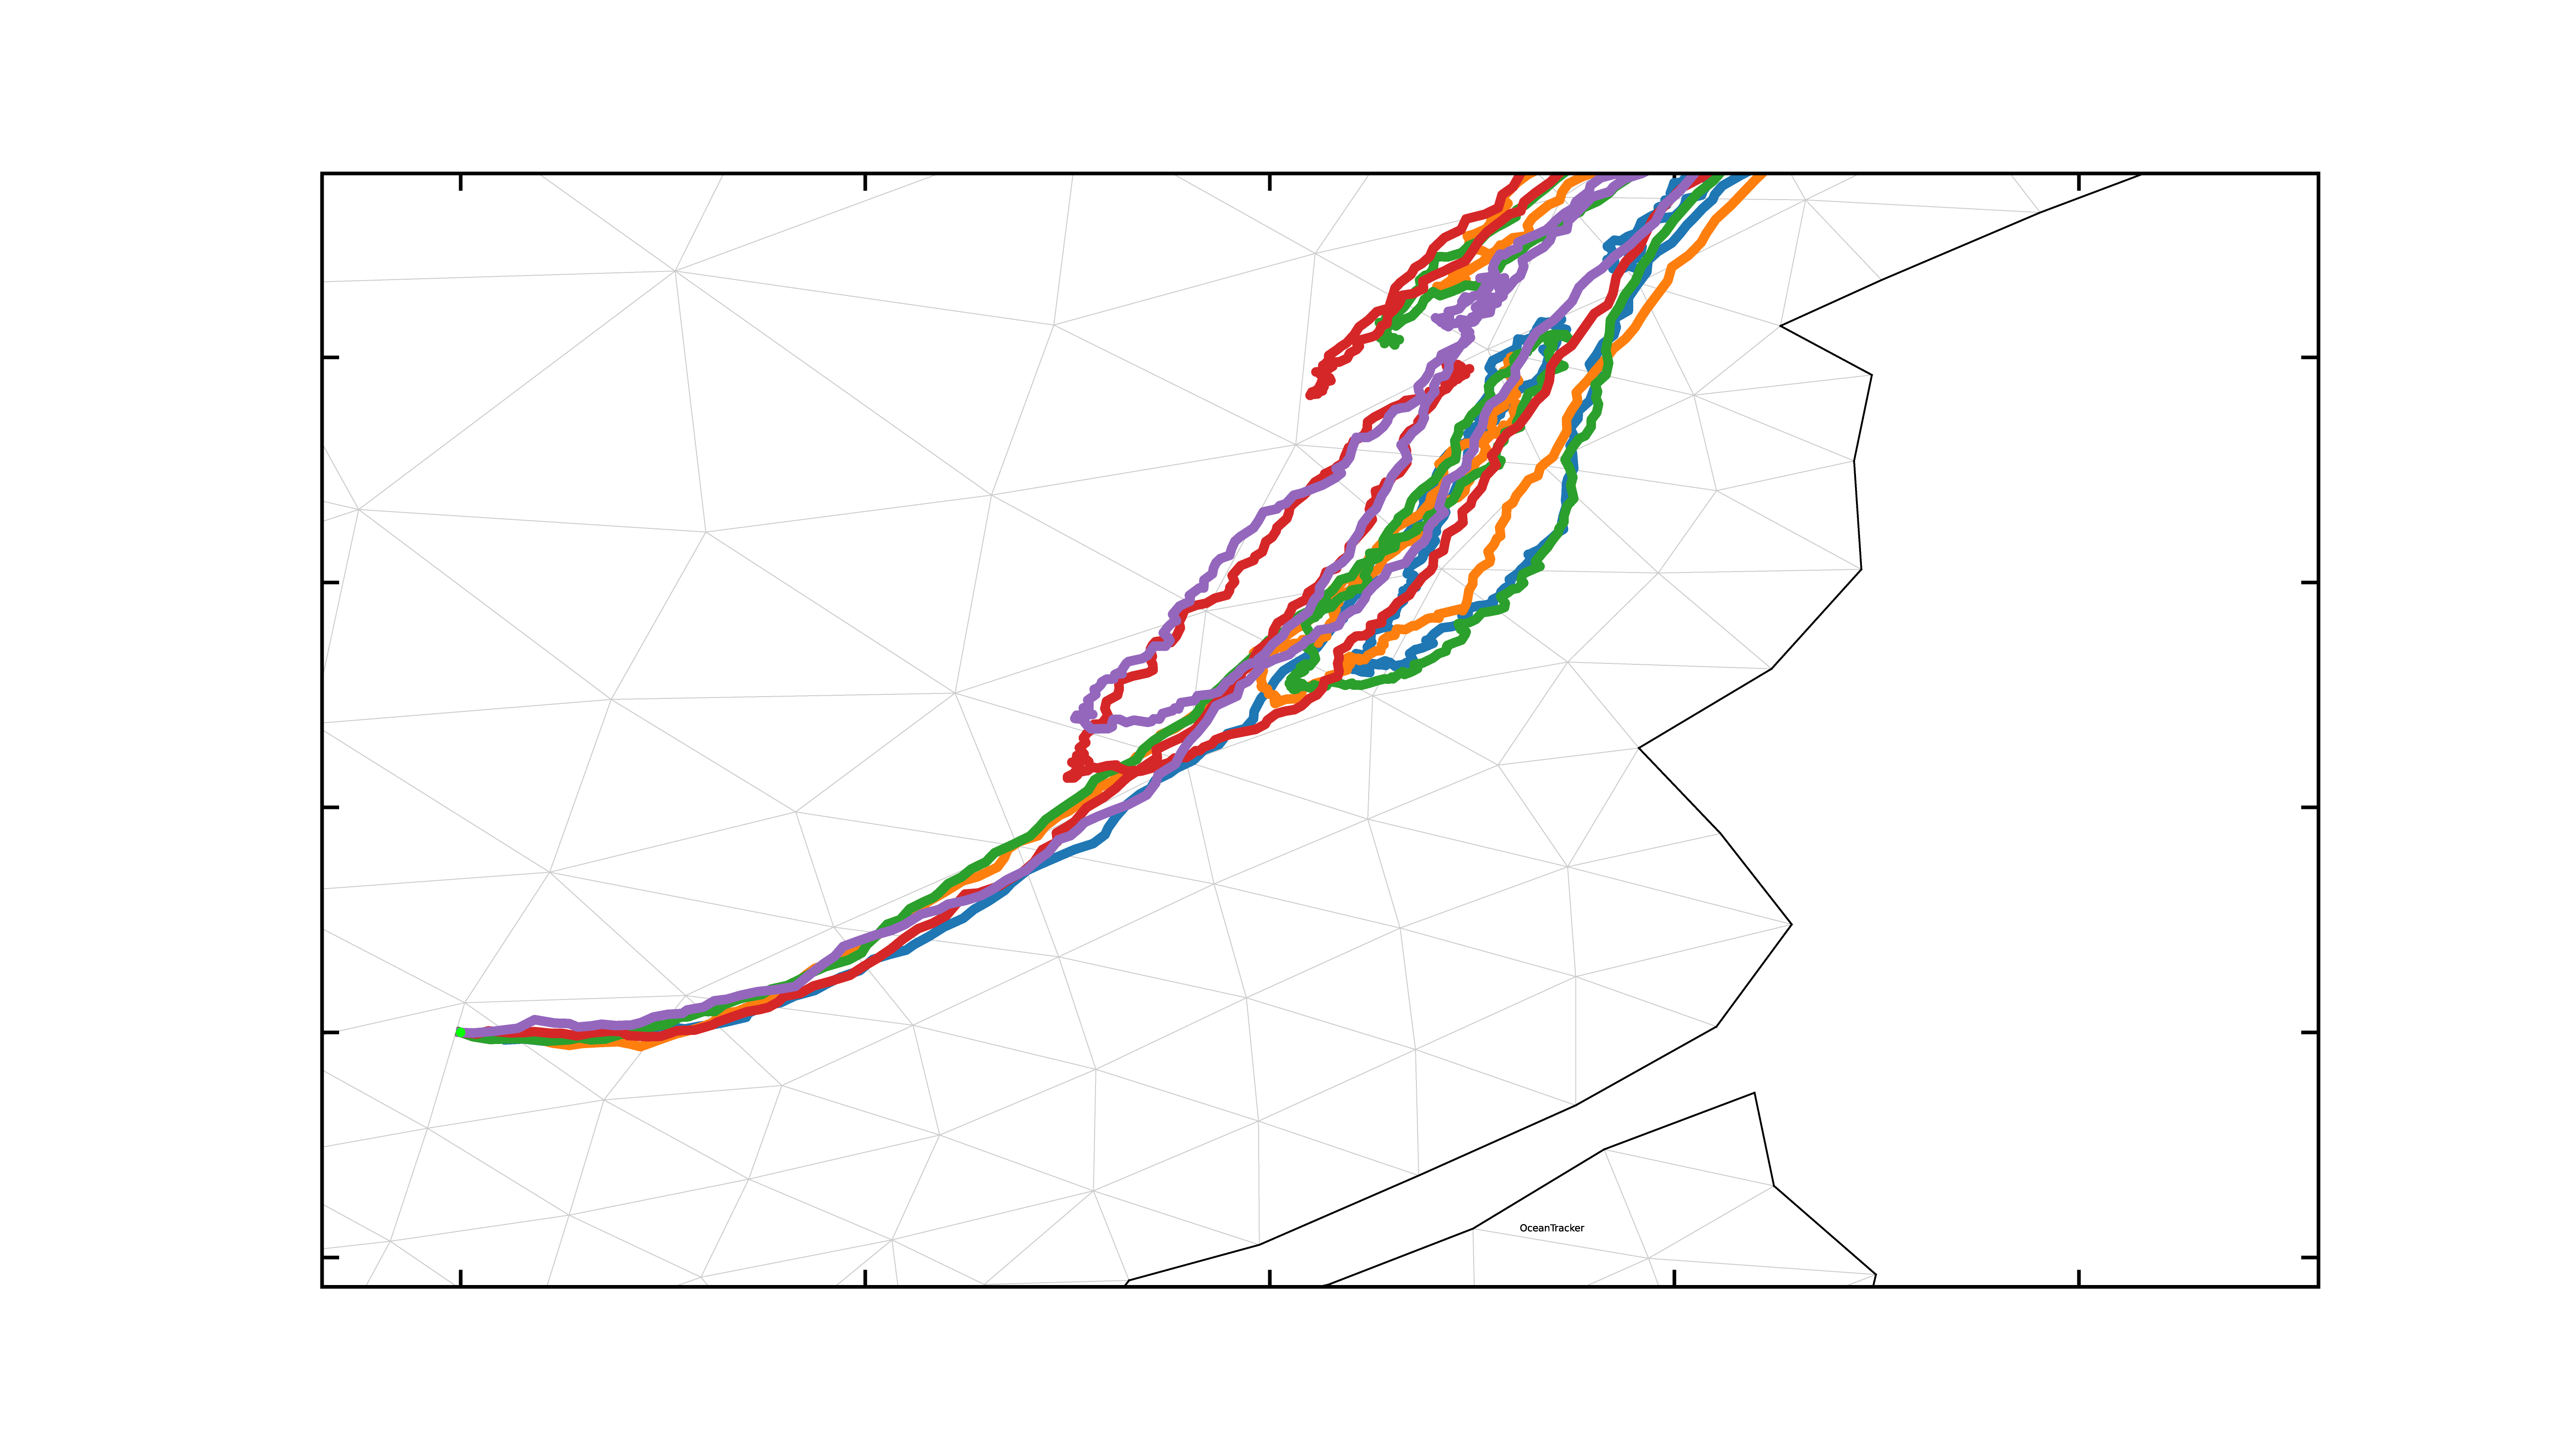
\includegraphics[width=\columnwidth]{Artboard 2.png}
    \caption{Particle Trackle visualisation - particle tracks on grid}
\end{figure}

\paragraph{data}
\begin{itemize}
    \item input is SCHISM output
    \item unstructured 3d grid of full estuary (geesthacht to helgoland with side-channels)
    \item (used) fields:
    \begin{itemize}
        \item temperature
        \item salinity
        \item water velocity 
    \end{itemize}
    \item full 2012 with 1h temporal- and ~5m spacial resolution
    \item year in reference to others
\end{itemize}
\begin{figure}
    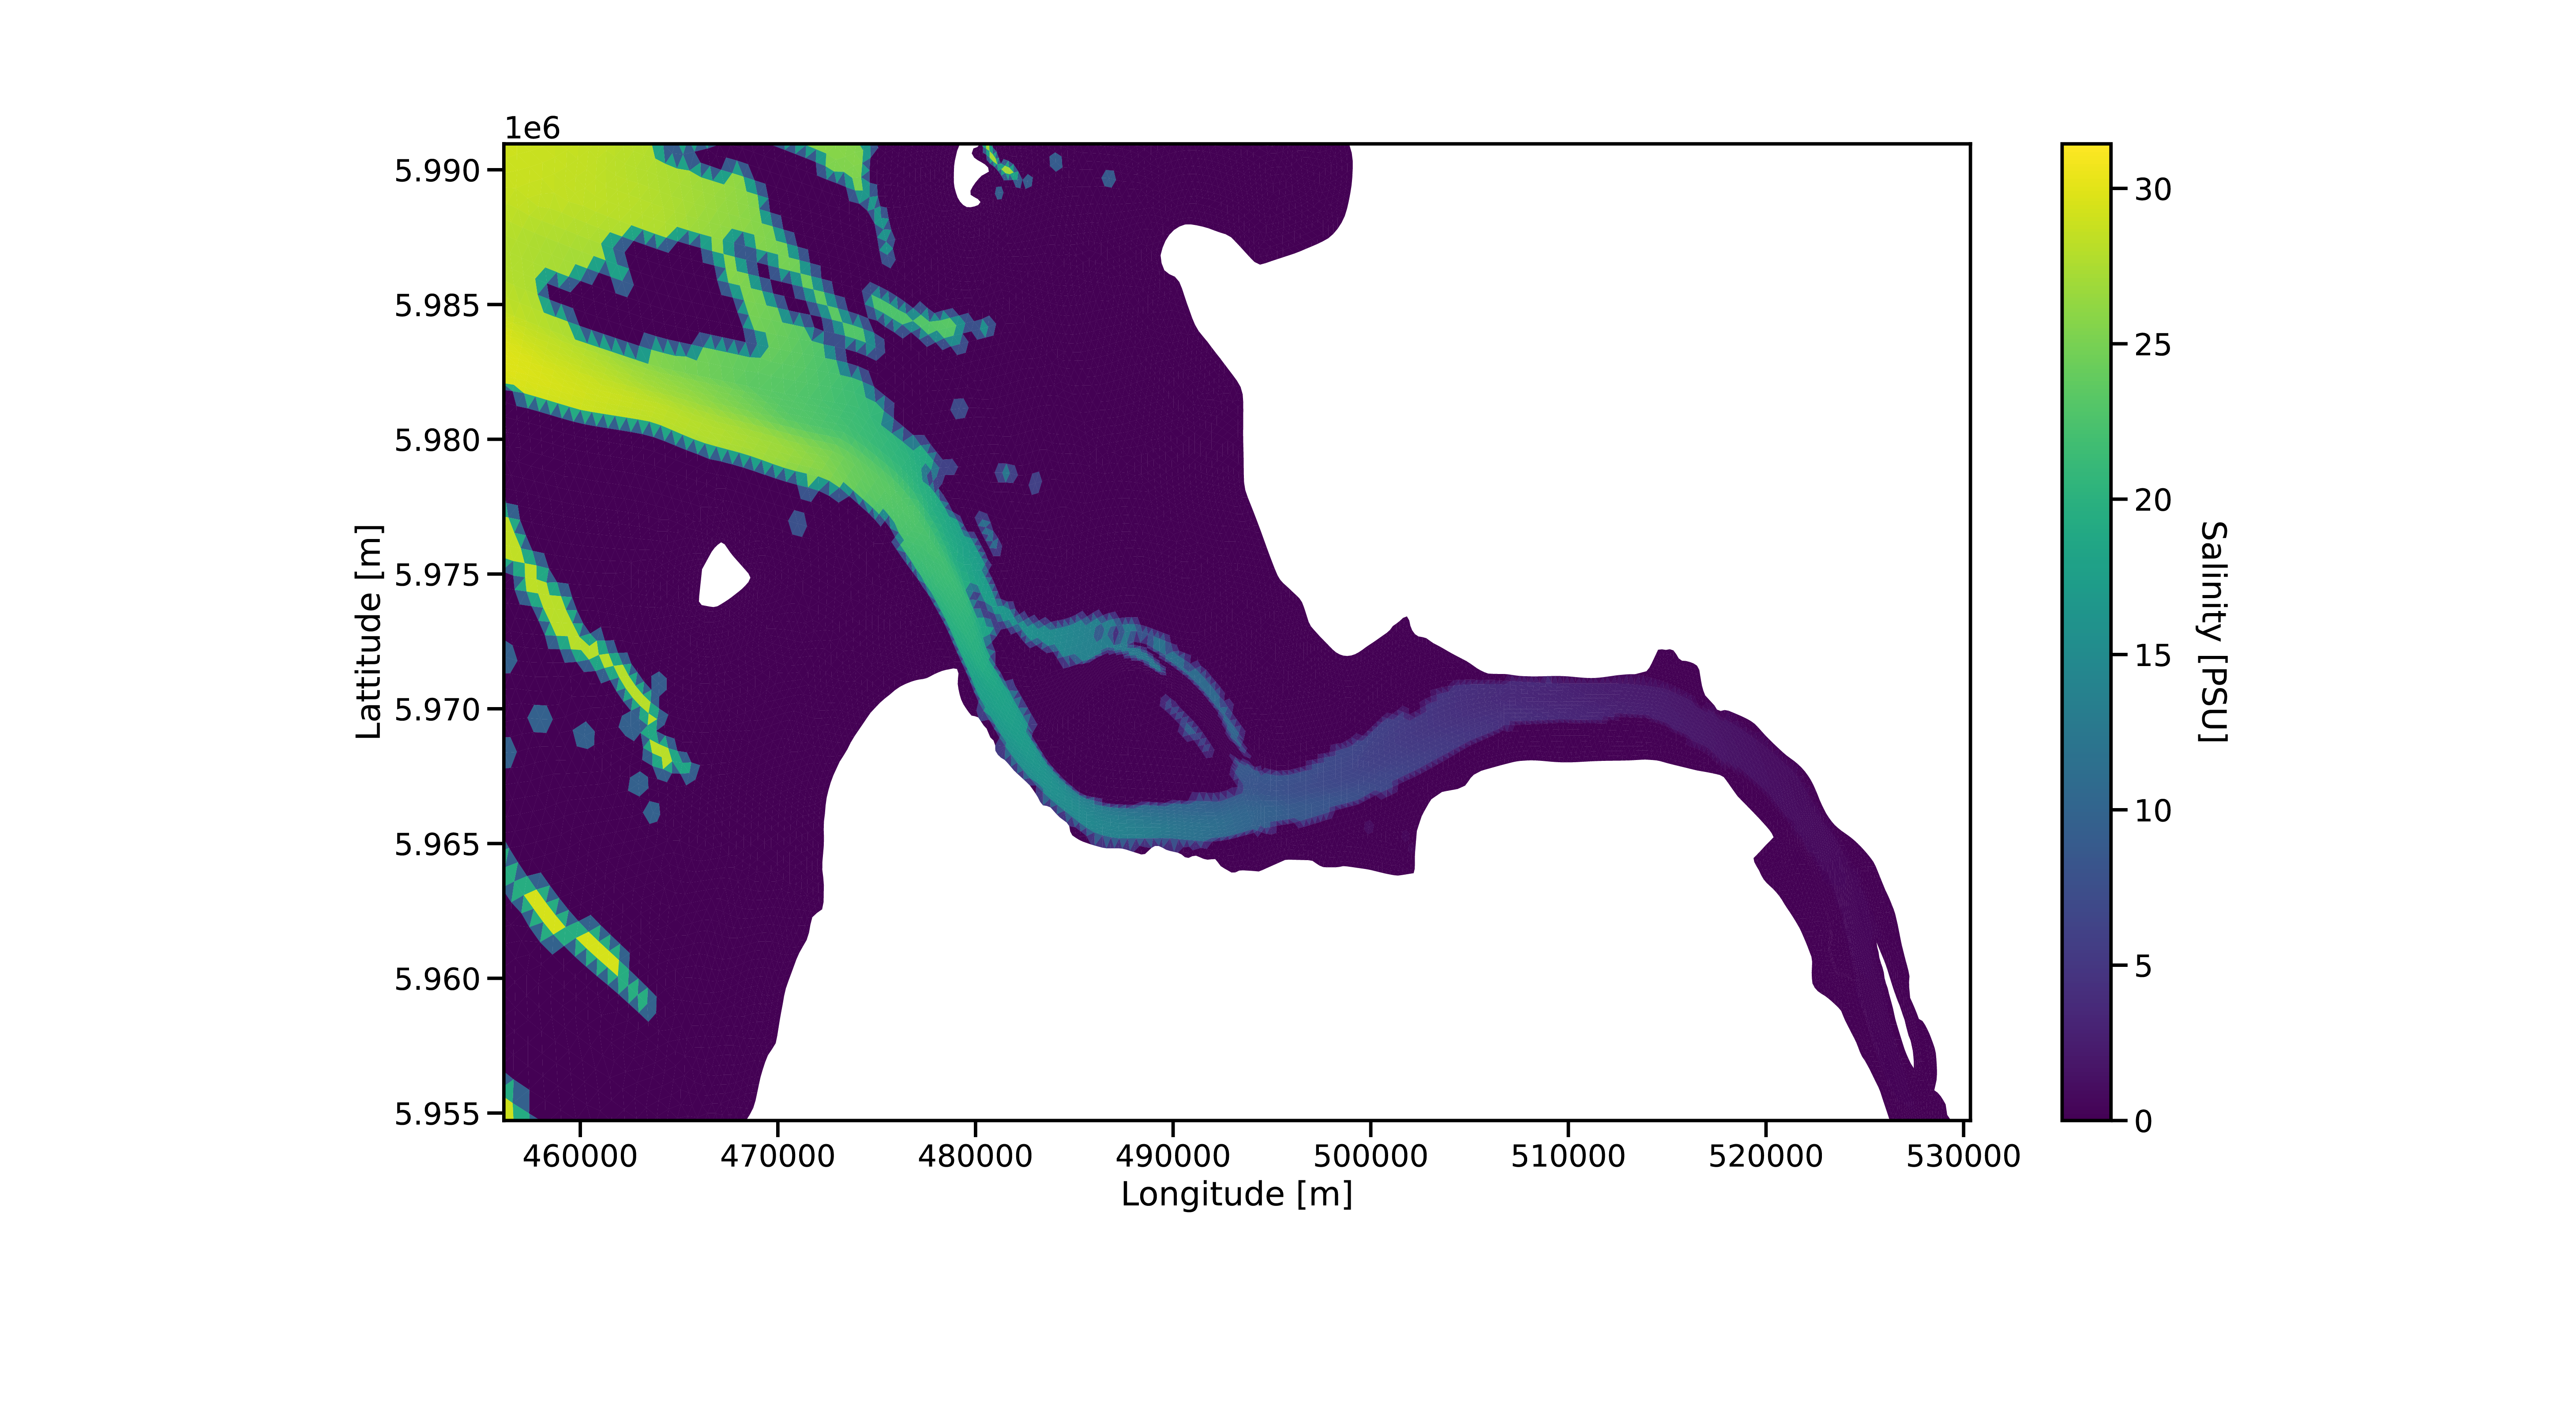
\includegraphics[width=\columnwidth]{Artboard 1.png}
    \caption{model domain visualization - full range grid including statistical polygons for later reference and example of a scalar field (e.g. temperature)}
    \label{fig:statistial polygons}
\end{figure}

\paragraph{bio-logical mechanisms represented in the model}
\begin{itemize}
    \item release
    \item splitting
    \item culling
    \item behavior
    \begin{itemize}
        \item sinking
        \item diel migration
        \item tidal migration
    \end{itemize}
    \item sedimentation/resuspension
\end{itemize}

\begin{figure}
    \centering
    \begin{minipage}{.4\columnwidth}
        \centering
        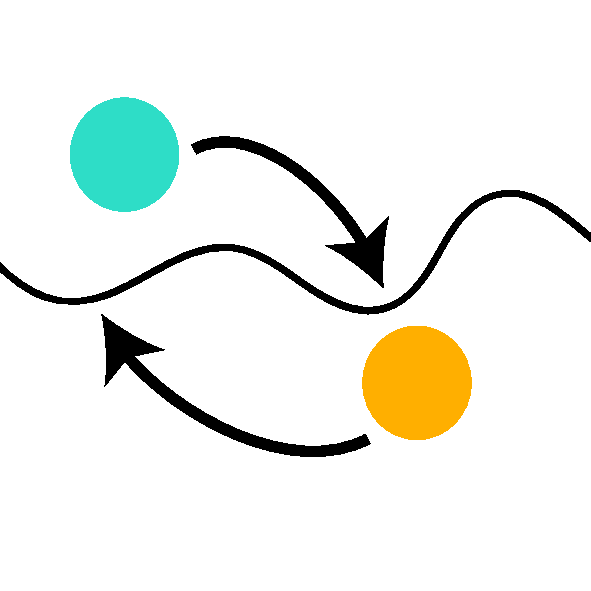
\includegraphics[width=.3\columnwidth]{picto resuspension.pdf}
    \end{minipage}
    \begin{minipage}{.4\columnwidth}
    \centering
        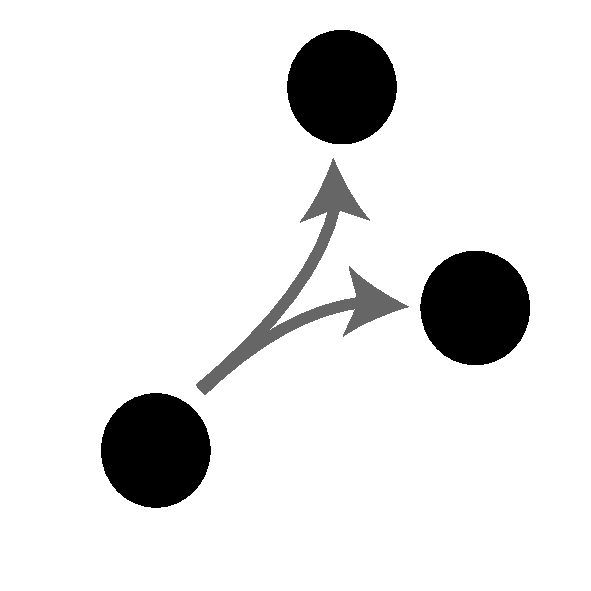
\includegraphics[width=.3\columnwidth]{picto splitting.pdf}
    \end{minipage}
    \caption{examples of pictograms for bio processes}
\end{figure}


\paragraph{Data Analysis}
\begin{itemize}
    \item Based on particle counts in statistical polygons \ref{fig:statistial polygons}
    \item statistical polygons roughly 100km in length
    \item calculation of particle "centroid" and whether particles are in a section of the estuary.
    \item successful retainment is judged by whether or not particles remain alive somewhere in the estuary after one year.
\end{itemize}
\begin{figure}
    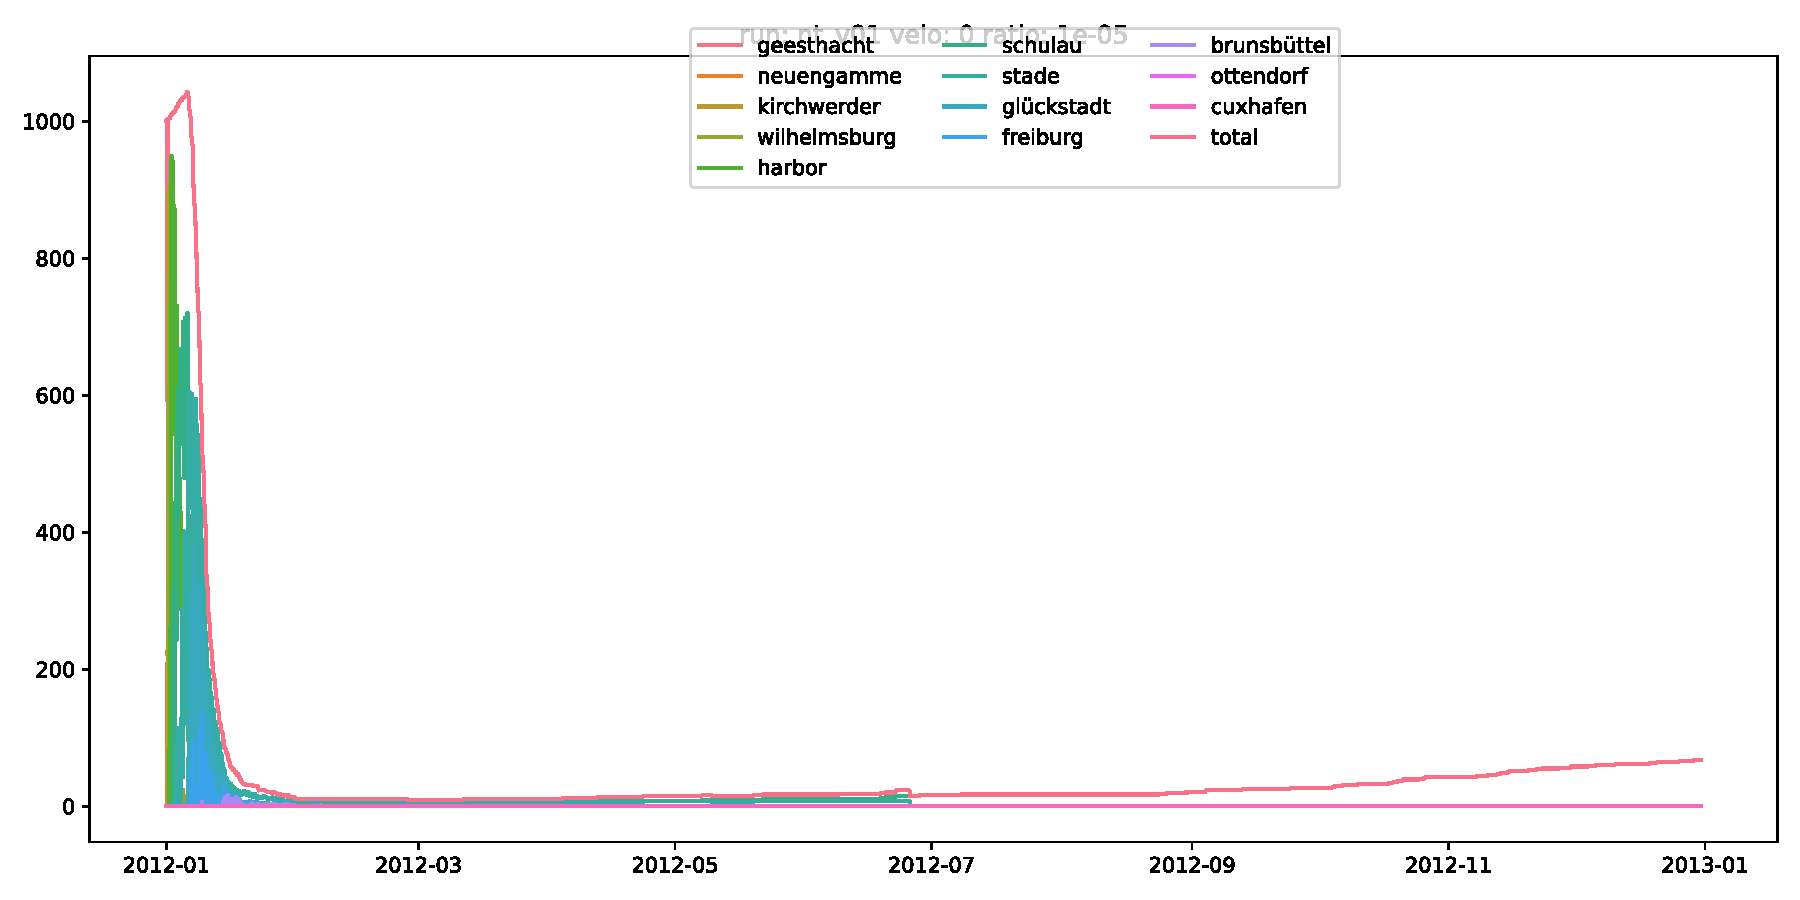
\includegraphics[width=\columnwidth]{fixed_particle_culling.pdf}
    \caption{Example 2d plot of particle counts, centroid and "retainment" threshold}
\end{figure}

\subsection*{Experimental configurations}

Two major setups with several minor configuration setups in relation to reference configurations
\begin{figure}
    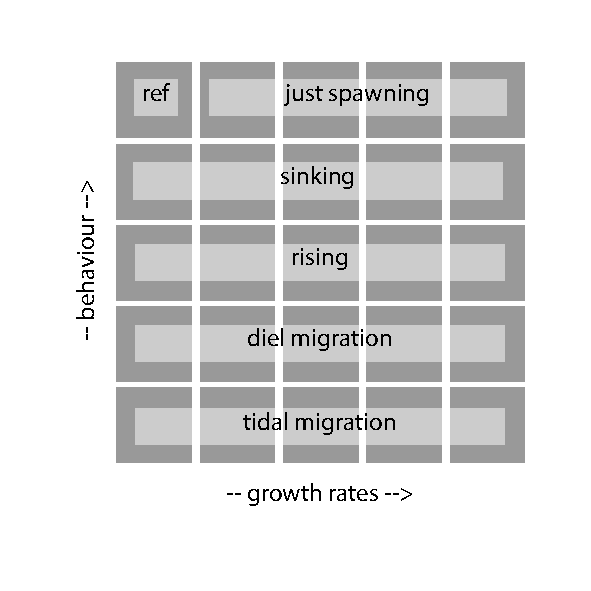
\includegraphics[width=\columnwidth]{plot experimental configuration.pdf}
    \caption{2d grid with boxes for the different cases/dimension. 
             Same structure as the later sensitivity analysis plot used \ref{fig:retention_results_SA}}
    \label{fig:experimental_configuration}
\end{figure}

\paragraph{reference run - dead\&passive}
\begin{itemize}
    \item no reproduction 
    \item no behavior just drifting
\end{itemize}

\paragraph{downstream retention}
\begin{itemize}
    \item studies retention mechanisms under different behavior/growth
    \item sensitivity analysis with the following dimensions
    \begin{itemize}
        \item growth rate 
        \item sinking
        \item diel migration
        \item tidal migration
    \end{itemize} 
    \item release location description
\end{itemize}


\paragraph{upstream migration}
\paragraph{downstream retention}

(Note: This is the "release downstream and check if we find some upstream" experiment)
\begin{itemize}
    \item studies reseeding mechanisms of upstream waters under different behavior/growth
    \item same SA dimensions as above
    \item release location description
\end{itemize}

\section*{Results}

\subsection*{downstream retention}

\begin{figure}
    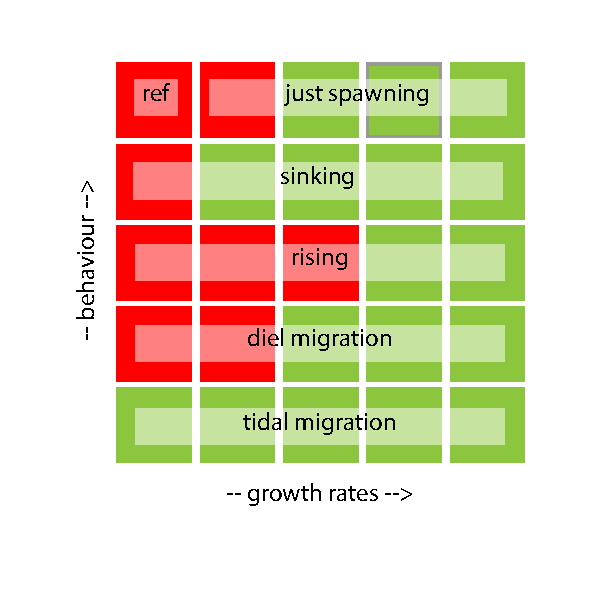
\includegraphics[width=\columnwidth]{plot results sa.pdf}
    \caption{2d grid with boxes for the different cases/dimension. 
             each box represents one configuration and whether they were able to retain by color code.
             I.e. a bunch of red and green boxes with axis labels}
    \label{fig:retention_results_SA}
\end{figure}

\begin{figure}
    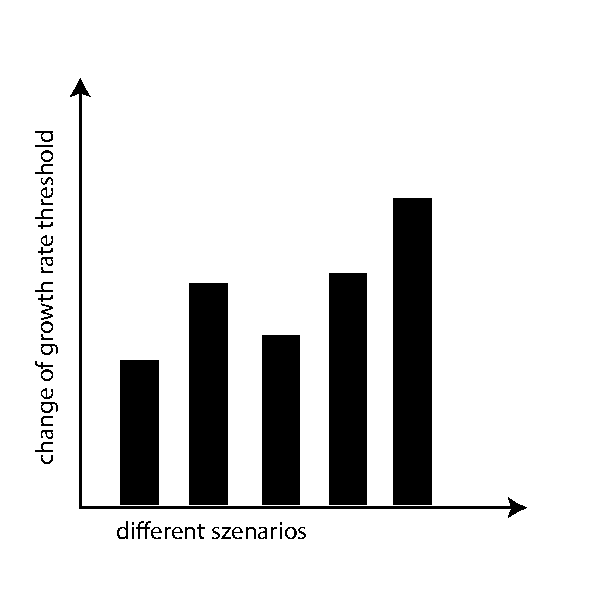
\includegraphics[width=\columnwidth]{plot result threshold change.pdf}
    \caption{bar plot of the $\frac{\partial \mu_{min}}{\partial v_{verticle}}$ relations}
    \label{fig:retention_results_dmu}
\end{figure}

\begin{itemize}
    \item discuss which configuration maintained a population and which not
    \item describe growth threshold under different behavior scenarios
    \item describe $\frac{\partial \mu_{min}}{\partial v_{verticle}}$ for sinking, diel-, tidal migration
\end{itemize}

\paragraph{reproduction dimension}
\begin{itemize}
    \item discuss which configuration managed to colonize upstream areas
    \item discuss threshold growth rates and the impact of behavior patters similar to above
\end{itemize}

\paragraph{Discuss Results}
contextualize the results 
\begin{itemize}
    \item doubling times of reproduction of threshold reproduction rates (for context)
    \item threshold reproduction rates in relation to "realistic" reproduction rates summer/winter - aka are these mechanisms sufficient to allow survival
    \item discuss effectiveness of migration behavior - most effective mechanisms should a priori be realized in nature 
    \item (once all results are done - check if we can make predictions that are experimentally testable. e.g. average sinking velocities)
    \item reseeding (with the preliminary results) is not possible - no upstream migration above the harbor aka non-tidal-dominated-areas
\end{itemize}


\section*{Discussion}
\begin{itemize}
    \item discuss limitation of the model
    \begin{itemize}
        \item simplified bottom/sediment interaction
        \item no "small object" representation e.g. vegetation or "rocks"
        \item simplistic bio representation. does not allow for precise quantification but only indicates bounds for values
        \item other minor issues - temporal resolution, particle out-of-bounds cases etc
    \end{itemize}
    \item discuss choice of particle tracking model compared to concentration based model
\end{itemize}



% \section*{What}
% 	\begin{itemize}
% 	\item Study retention mechanism of planktion
% 	\item Theoretical approach with an mixed Eulerian Lagrangien model
% 	\item Demonstrate that "passive" organisms aka particles will ultimatly drift downsteam until and be removed from the estuary
% 	\item Study different retention patterns
% 	\begin{itemize}
% 		\item [placeholder]
% 	\end{itemize}
% 	\item Elbe
% 	\item "alive" particles
% 	\end{itemize}
% 
%  
% 
% \section*{Why}
% \begin{itemize}
% 
% \item particle without retention mechanism - aka "full plankton mode" would drift
%   downstream.
%   change in relative stream position induces changes in salinity
%   hence moves out of ideal salinity zone which results in unfavourable conditions
%   can result of an strong case of death or being outcompeted.
% \item the existance of specialized plankton organism [cite] that only live the tidal section of the river
%   also implies the existance of retention mechanisms since in their case a "reseeding" process from up- or downstream is not possible
% 
% \item the avoid extinction retention mechanism need to be present
%   [cite chesterfield bay study][cite zooplankton study]
% 
%  \item first theories have been tested but so far exclusively with "dead" particles
%   no biophychemical coupled systems
%   "dead" system are of limited explanatory power.
%   concepts like "re-seeding" can not be tested
%   reproduction and dying acts as an amplification in favourable conditions
% 
% \end{itemize}
% 
% \section*{How}
% \begin{itemize}
% 
% 	\item	SCHISM hydrodynamic model coupled with OT 
% 	\begin{itemize}
% 		\item offline coupled hyrdro to lagrangien particle tracker
% 		\item Euler by SCHISM
% 		\item Lagrangien by OceanTracker
% 		\item high speed (24h a 1e6 particles @ 2 minutes)(faster then any model before!)
% 		\item Including biochemical mechanisms
% 	\end{itemize}
% 
% 	\item Ideas to discuss the outcome Results: 
% 	\begin{itemize}
% 		\item Compare retention performance with distribution patterns
% 		\begin{itemize}
% 			\item This will most probably not possible as there is to little 
% 				  observation data to compare spacial distributions
% 			\item 
% 		\end{itemize}
%   		\item Compare "alive" to "dead"
% 	\end{itemize} 
% 
% \end{itemize}